\chapter{Resultados}
\label{cap:resultados}

\section{Métricas e Medição}
  Para medir o tempo  de execução e processamento  do programa utilizamos dois softwares. Principalmente o \textit{gprof} para medir a performance das funções separadamente e o gnu \textit{time} para medir o tempo total de execução dos programas.

  Os testes foram executados em um Ubuntu 17.10, x64, AMD Fx-6100 six-core processor, 8gb de ram e uma placa de vídeo Nvida Geforce GTX 550TI, com 192 núcleos e 1024 Mb de memória. O número máximo de threads simultâneas na CPU é de 6 enquanto na GPGPU é 32 vezes esse valor, são 192 execuções paralelas no máximo.

  O grafo \ref{fig:grmonty-performance} apresenta a ordem e tempo consumido em cada chamada de função no grmonty pré-otimização, nele é evidente o alto custo para se realizar o  \textit{track\_super\_photon}. Já o grafo \ref{fig:cudamake} tenta mostrar o mesmo grafo só que para o código já portado para CUDA, porém a ferramenta utilizada a gprof, não foi capaz de medir a porcentagem de tempo que foi utilizada em funções que rodaram na GPGPU, mas mesmo assim é possível olhar a quantidade de vezes que a função foi chamada - no caso da  \textit{track\_super\_photon} ela foi chamada mais de 1.100.000 vezes para um N de 100 mil.

  \begin{figure}[!h]
    \centering
    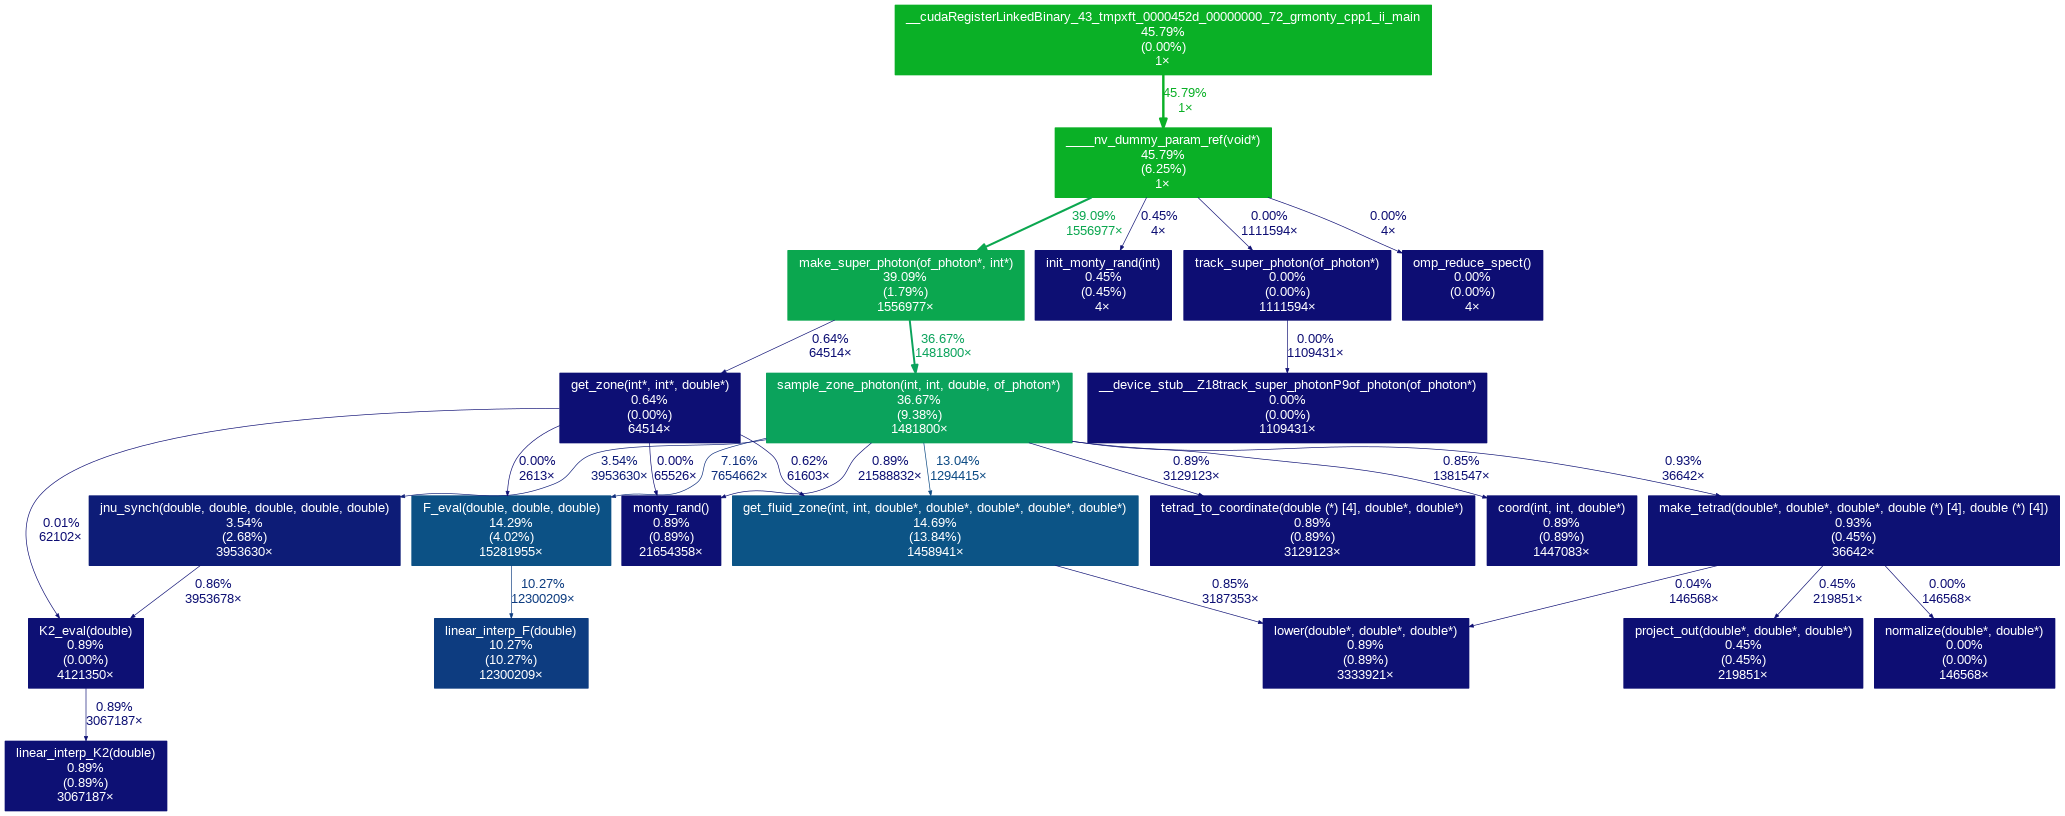
\includegraphics[width=1\textwidth]{cuda_make.png}
    \caption{grafo de chamadas e porcentagem de tempo utilizado por função do grmonty em CUDA}
    \label{fig:cudamake}
  \end{figure}

  O grafo em \ref{fig:cudamake} é um recorte do grafo completo, já que ao se executar chamadas de código CUDA várias outras auxiliares, internas a arquitetura CUDA são invocadas, tal fato aumenta em muito o grafo e pode trazer um comprometimento a sua legibilidade, devido a este fato seu grafo esta suprimido aqui, mas está presente no apêndice.

\section{Comparações}
  O gráfico abaixo \ref{fig:magica} demonstra como o grmonty performa e como performa após ter parte de seu código portado para CUDA, conforme o número de fótons N cresce. Os pontos foram gerados executando-se as duas aplicações -  a primeira versão completamente na CPU e a segunda com parte do processamento na GPGPU - Os valores de N vão de 0 a 100 mil pulando de 5mil em 5mil.

  É fácil perceber que a versão em CUDA apresenta um tempo de execução bem menor que sua contrapartida na CPU. A diferença tende a $1/3$, a versão em CUDA só toma 1 terço do tempo que a em GPU. É possível perceber também, olhando para o início do gráfico, quando N vale 0, que a versão em GPGPU possui um overhead maior, um maior tempo de inicialização que a outra versão.

\begin{figure}[!h]
  \centering
  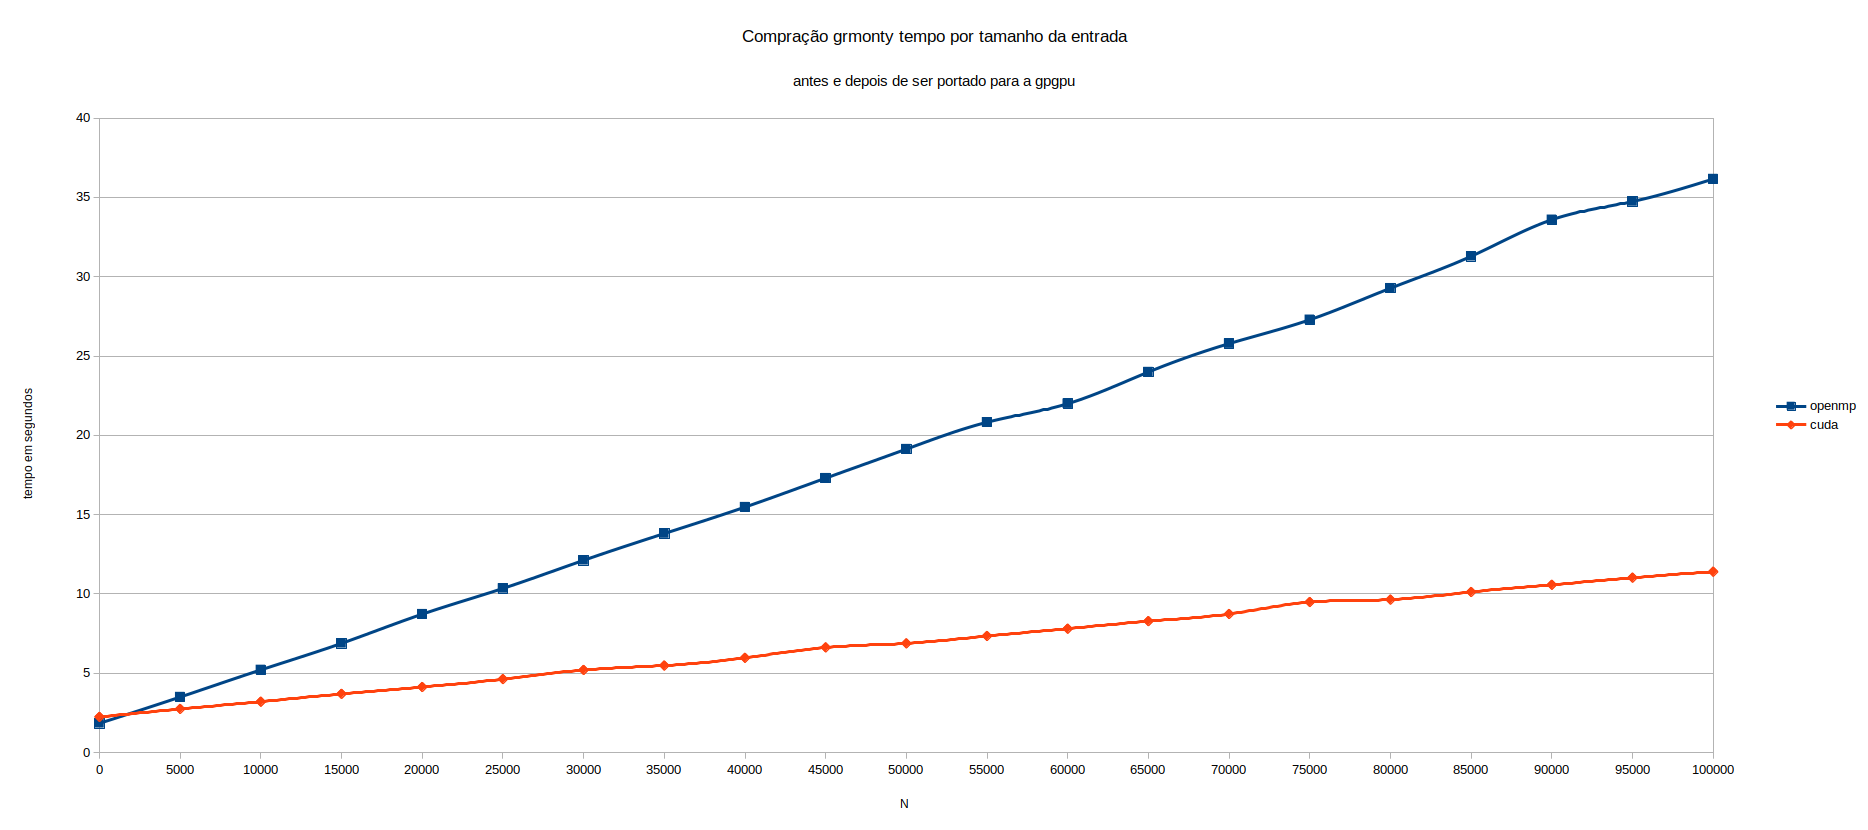
\includegraphics[width=1\textwidth]{magica.png}
  \caption{gráfico comparativo, antes e depois da otimização}
  \label{fig:magica}
\end{figure}
